\subsection{Tokenization}
\label{sec:parsing-tokenization}

Given a grammar $G$ and a sentence $S$, the tokenization\footnote{we use the term tokenization as a combination of substring identification and retrieval of LTAG/DUDES from the given grammar.} phase partitions $S$ in a ordered sequence of regular expressions $\{\pi\}$, each one referring at least one elementary LTAG/DUDES in $G$.
%
The \texttt{Tokenizer} is the software component responsible to execute the tokenization phase

In Figure~\ref{fig:tokenization-sample} we show some notable execution of the tokenization phase.
%
Every time the \texttt{Tokenizer} is invoked on $S$ with $G$, it looks in $S$ for the \textbf{longest regular expression} matching an entry in $G$.
%
Once the regular expression has been matched, the \texttt{Tokenizer} emits a \textit{token} $t$, that is an element defined as follows:

\begin{equation}
\label{eqn:token}
token:=(regexp,pos,candidates)
\end{equation}

where
$regexp$ is the regular expression matched in the substring of $S$ starting at position $pos$, and
$candidates$ is the list of LTAG/DUDES in $G$ associated with $regexp$.

Notice that $pos$ is recorded inside a token because it can be used by the parsing algorithm to always be able to locate a token inside the sentence.

\begin{figure}[tp]
	\label{fig:tokenization-sample}
	\centering
	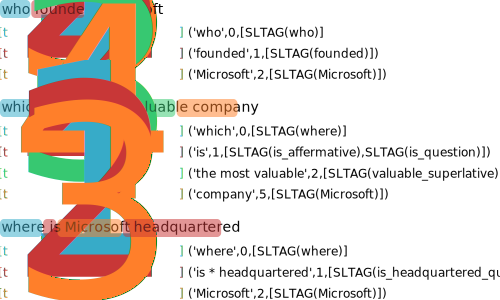
\includegraphics[width=0.8\columnwidth]{./fig/tokenizer-sample}
	\caption{An example of the tokenization phase. In this figure, we denote with \textit{LTAG/DUDES('word')} the elementary LTAG/DUDES associated to the entry \textit{'word'}.}
\end{figure}

The \texttt{Tokenizer} is a stateful component, hence it leverages convenient data structures to encapsulate its state.
%
The most important one is the buffer, that records whether or not a word in $S$ has been already tokenized.

In Algorithm~\ref{alg:tokenizer} we show the pseudocode of the tokenization process.
%
The \texttt{Tokenizer} exposes a convenient API to iterate over tokens, that is clearly inspired to the well known \textit{API provided by Java generic iterators}.

\begin{algorithm}[t]
	\SetKwProg{Fn}{Function}{}{}  
	%\Fn{nextTokenizable()}{
	%\For{$b\in buffer$}{
	%	\If{$b.tokenizable\; \& \; b.tokenized$}{
	%		\KwResult{$buffer.index(b)$}
	%	}
	%}
	%\KwResult{$-1$}
	%}	
	
	\Fn{hasNext()}{
	%\KwResult{$nextTokenizable() \neq -1$}
	}
	
	\Fn{next()} {
		$start \leftarrow nextTokenizableIndex()$ \\
		\If{$\neg start1$}{
			\KwResult{$NULL$}
		}
	
		$end \leftarrow start$ \\
		
		\While{$end < buffer.size$}{
			$elem \leftarrow buffer.get(end)$ \\
			\If{$elem.tokenized = False$}{
				$tmpRegexp.concat(elem.word)$ \\
			}
			$matchType \leftarrow grammar.matchMode(tmpRegexp)$ \\
			\If{$matchType = FULL$}{
				$candidates \leftarrow grammar.getAll(tmpRegexp)$ \\
				$regexp \leftarrow tmpRegexp$ \\
				$buffer.get(end).tokenized \leftarrow True$ \\
				\If{$returnFirstFull = True$}{
					break
				}
			}
			\ElseIf{$matchType = NONE$}{
				break
			}
			\ElseIf{$matchType = PART$}{
				$buffer.get(end).tokenized \leftarrow True$ \\
			}
			\ElseIf{$matchType = STAR$}{
				\If{$consuming = False$}{
					$consuming \leftarrow True$ \\
					$startConsuming \leftarrow end$ \\
				}
				\Else{
					\If{$end = buff.size - 1$}{
						$consuming \leftarrow False$ \\
						$end \leftarrow startConsuming - 1$ \\
						$returnFirstFull \leftarrow True$ \\
					}
				}
			}
		
			$end \leftarrow end + 1$ \\
		}
	
		\KwResult{$Token(regexp,pos,candidates)$}		
	}
	\caption{Pseudocode of the \texttt{Tokenizer} API.}
	\label{alg:tokenizer}
\end{algorithm}

Some functions in Algorithm~\ref{alg:tokenizer} have not been formally defined because they are pretty self-explanatory or have been partially introduced in previous sections.
For reader's sake, we briefly describe the most important ones here. 

Recall that an entry $e$ in grammar $G$ is a tuple

\begin{equation}
\label{eqn:grammar-entry}
e:=(regexp,LTAG/DUDES)
\end{equation}

where
$regexp$ is the regular expression representing the syntactic usage of $e$ in a sentence, and
$LTAG/DUDES$ is the elementary LTAG/DUDES in $G$ representing the syntax and semantics of $e$.

\texttt{grammar.matchMode(str)} matches the specified string \textit{str} against the entries in grammar. 
%
The following matching modes have are defined:
%
\begin{itemize}
	\item[FULL] the grammar contains an entry matching str, and no entry starting with it. 
	For example, the entry \textit{'Microsoft'} matches is such way the grammar $\{who,founded,Microsoft\}$.
	
	\item[PART] the grammar contains no entry matching str, but an entry starting with it.
	For example, the entry \textit{'founders'} matches is such way the grammar $\{who,are,the,founders of,Microsoft\}$.
	
	\item[STAR] the grammar contains no entry matching str, but a entry starting with it and consuming the last part of it with the \textit{star-operator (*)}.
	For example, the entry \textit{'is'} matches is such way the grammar $\{where,is\;*\;headquartered,Microsoft\}$.

	\item[NONE] the grammar contains no entry matching str in one of the previous mode.
	For example, the entry \textit{'Google'} matches is such way the grammar $\{who,founded,Microsoft\}$.
\end{itemize}

\texttt{grammar.getAll(str)} retrieves from the grammar all the SLTAGs associated with a regular expression matching \textit{str} in \texttt{FULL} mode.